\documentclass{report}
\usepackage{graphicx} % Required for inserting images
\usepackage[italian]{babel}
\usepackage{tikz}
\usepackage{hyperref}
\usepackage{amsmath}
\usepackage{xcolor}

\definecolor{darkgreen}{rgb}{0.0, 0.5, 0.0}


\title{Introduzione al Cloud}
\date{Parte III}

\begin{document}

\maketitle

\tableofcontents
\newpage

\chapter{Introduzione}
Gli avanzamenti tecnologici degli ultimi anni hanno cambiato 
la nostra società: nella società in cui viviamo oggi la tecnologia è 
pervasiva (\textit{Internet of Things}), abbiamo tutto quello che avevamo
prima però smart; inoltre il cluod viene largamente utilizzato per storage o computing

$ \rightarrow $ \textbf{tutto questo
signfica flusso di dati da me a fuori}.

\subsubsection{Vantaggi:}
\begin{itemize}
    \item \textcolor{darkgreen}{+} Migliori meccanismi di protezione
    \item \textcolor{darkgreen}{+} Resilienza rispetto a malfunzionamenti
    \item \textcolor{darkgreen}{+} Miglior prevenzione e risposta (dato che il sistema è smart, può inividuare certe anomalie e prevenire 
    un attacco che sta per accadere)
\end{itemize}

\subsubsection{Svantaggi:}
\begin{itemize}
    \item \textcolor{red}{-} Maggiore complessità: basta una singola porta per accedere a tutto
    \item \textcolor{red}{-} La stessa velocità che abbiamo in positivo per le funzionalità, ce l'hanno anche gli attaccanti.
    \item \textcolor{red}{-} Incremento di danni e violazioni
    \item \textcolor{red}{-} Perdita di controllo su dati e processi
\end{itemize}

Due ulteriori problemi:
\begin{itemize}
    \item \textcolor{red}{-} devices vulnerabili ad attacchi esterni
    \item \textcolor{red}{-} devices che contengono dati sensibili che, se attaccati, possono essere portati fuori
\end{itemize}

\subsubsection{Sicurezza\dots un problema complesso}
La sicurezza è un problema complesso poichè richiede una soluzione a molti problemi (protezione delle infrastrutture, dei dati, dei dispositivi, della rete, malware, \dots).

\subsubsection{Sistema Smart}
Ciò che rende un sistema \textit{smart} è la capacità di acquisire, analizzare e processare dati per acquisire conoscenza 
da iniettare nuovamente nel sistema 

$ \rightarrow $ prevedibilità dell'utente

\section{Cloud computing}
Il cloud permette a organizzazioni e utenti finali di avvalersi di servizi esterni per 
immagazzinare, processare e accedere ai loro dati.
\begin{itemize}
    \item \textcolor{darkgreen}{+} Altà configurabilità
    \item \textcolor{darkgreen}{+} Dati e servizi sono sempre disponibili
    \item \textcolor{darkgreen}{+} Scalabilità
\end{itemize}

$ \rightarrow $ gli utenti perdono il controllo dei loro dati, necessità di nuove soluzioni di sicurezza per \textbf{proteggere i dati e 
processarli in maniera sicura nel cloud}.

\subsubsection{Cloud: oggi}
Ad oggi i cloud providers applicano misure di protezione solamente da eventuali utenti esterni (protezione rispetto al perimetro).
Due scenari possibili:
\begin{itemize}
    \item \textbf{piena fiducia} nel cloud provider in quanto ha pieno accesso ai dati
    \item proteggiamo i dati anche dai cloud provider ma abbiamo \textbf{funzioni limitate}, uso del provider solo come storage
\end{itemize}

\subsubsection{Cloud: nuova visione}
Si vogliono adottare soluzioni che offrono garanzie di protezione dando al \textit{data owner} sia pieno controllo dei dati che alta funzionalità su di essi (sia 
sicurezza verso l'esterno che verso il cloud provider stesso).
\begin{itemize}
    \item \textbf{client-side trust boundary:} solo i comportamenti del client dovrebbero essere considerati fidati
\end{itemize}


\section{Data protection}
Proteggere i dati non è semplice, bisogna minimizzare l'esposizione ricordandosi:
\begin{itemize}
    \item correlazione tra diverse sorgenti
    \item esposizione indiretta di informazioni sensibili (ciò che potrebbe portare inferenza)
    \item non identificabilità $ \neq $ anonimato
\end{itemize}

\chapter{Caratteristiche delle sfide di Protezione dei Dati nel Cloud}
\section{Le tre dimensioni del problema}
Queste sono le tre dimensioni del problema \textit{privatezza e protezione nel cloud}.
Non c'è una definizione di sicurezza assoluta, dipende sempre da quella richiesta e dal contesto applicativo.
\begin{figure}[ht]
    \centering
    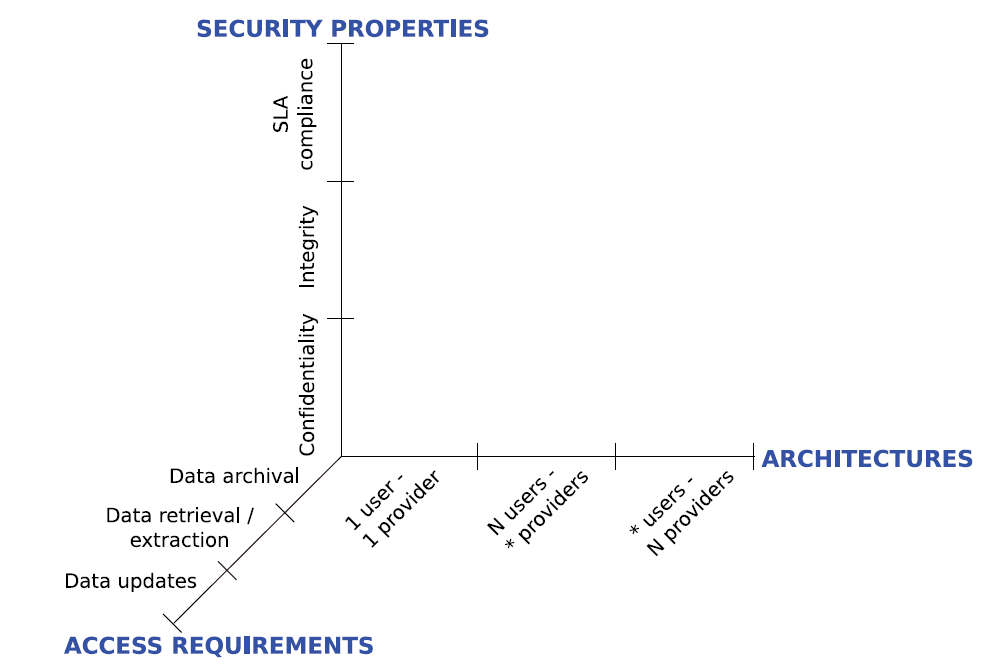
\includegraphics[width=1\linewidth]{images/3 dimensioni.png}
\end{figure}

\subsection{Proprietà di sicurezza (CIA)}
\begin{itemize}
    \item \textbf{ Confidenzialità:}
    \begin{itemize}
        \item protezione dei dati archiviati nel cloud
        \item autenticazione fatta non su chi l'utente è ma sulle proprietà che ha (certificazioni); \textit{se devo andare in biblioteca, non serve dire chi sono ma solo che
        sono uno studente della statale}.
        \item protezione rispetto alle azioni che può fare un utente (confidenzialità sulla query)
    \end{itemize}
    \item \textbf{Integrità:} per essere integro il dato deve essere corretto, completo e fresco (\textit{up-to-date})
    \begin{itemize}
        \item integrità rispetto ai dati archiviati nel cloud
        \item integrità rispetto alla computazione e ai risultati delle queries: è molto più difficie garantirla in computazione,
        per questo motivo si aggiungono punti di controllo/si pongono domande di cui si sa già la risposta 
    \end{itemize}
    \item \textbf{SLA compliance (Server Level Agreement:)}
    indica l'\textit{availability} nel cloud, quindi non soffrire di negazione del servizio; gli utenti devono poter fare sempre ciò per 
    cui sono autorizzati.
\end{itemize}

\subsection{Access requirements (funzionalità richieste)}
\begin{itemize}
    \item \textbf{Archivio dati:}
    \begin{itemize}
        \item operazioni di upload/download
        \item protezione dei dati in storage (devo garantire che i file che ho memorizzato fuori siano protetti);
        se cripto, cripto a livello di file.
    \end{itemize}
    \item \textbf{Recupero ed estrazione dei dati:}
    voglio avere la capacità di eseguire delle query
    \begin{itemize}
        \item supporto per un livello di granularità più fine
        \item protezione della computazione della query (confidenzialità della query e integrità del risultato)
    \end{itemize}
    \item \textbf{Data update:}
    In questo contesto ho dei dati dinamici: 
    \begin{itemize}
        \item devo supportare operazioni di insert/update (granularità più fine)
        \item protezione della confidenzialità delle azioni, poichè potrebbero essere osseravti i cambiamenti
    \end{itemize}
\end{itemize}

\subsection{Architetture}

\begin{itemize}
    \item \textbf{1 user - 1 provider} (caso più semplice)
    \begin{itemize}
        \item protezione dei dati in storage
        \item granularità a livello di recupero dati
        \item privatezza e integrità delle query
    \end{itemize}
    \item \textbf{n users - * providers:}
    \begin{itemize}
        \item autorizzazione e controllo dell'accesso
        \item gestione di scritture multiple
    \end{itemize}
    \item \textbf{* users - n providers:} caso in cui ho diverse sorgenti dati che devono fare computazione insieme
\end{itemize}

\subsection{Combinazione delle dimensioni}
Ogni combinazione delle istanze delle tre dimensioni, identifica nuovi problemi; le proprietà di sicurezza da garantire
dipendono dai requisiti di accesso e sulle assunzioni di fiducia (\textit{trust assumption}) sui provider.

I providers possono essere:
\begin{itemize}
    \item \textbf{\textit{honest-but-curious}:} trusted rispetto all'affidabilità del servizio ma non trusted rispetto alla confidenzialità (sbircia nei dati)
    \item \textbf{\textit{lazy}:} in questo caso anche problema di integrità, provider che non svolge correttamente il suo compito (es: ritorna query incomplete per risprmiare risorse)
    \item \textbf{\textit{malicious}:} maggiore problema di integrità, dall'altra parte c'è qualcuno (non solamente il provider stesso) che fa uno sforzo per compromettere i dati
\end{itemize}

\chapter{Digital Data Market}
Vi sono diversi data owner che contribuiscono a uno spazio dati comune, per poi fare analisi.
Il problema è che i dati possono essere sensibili, bisogna capire il livello di protezione.
\begin{figure}[ht]
    \centering
    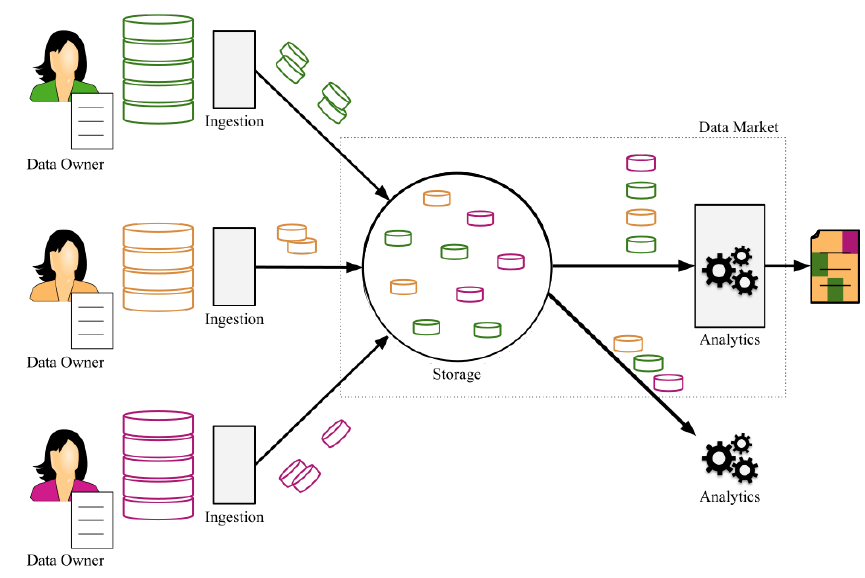
\includegraphics[width=1\linewidth]{images/digital data market.png}
\end{figure}

\subsubsection{Dimensioni del problema:}
\begin{itemize}
    \item \textbf{Comprensione dei requisiti:} la politica è difficile da controllare. 
    
    \textit{Sticky policy:} la politica dovrebbe essere attaccata ai dati (non c'è certezza)
    \item \textbf{Tencologie di applicazione (enforcing):}
    \begin{itemize}
        \item \textit{Data wrapping}: livello crittografico, può essere invertito
        \item \textit{Sanitizzazione}: dati vengono sanitizzati, non può essere invertito
    \end{itemize}
    \item \textbf{Fasi di applicazione:} \textit{ingestion, storage, analytics}
\end{itemize}

\begin{figure}[ht]
    \centering
    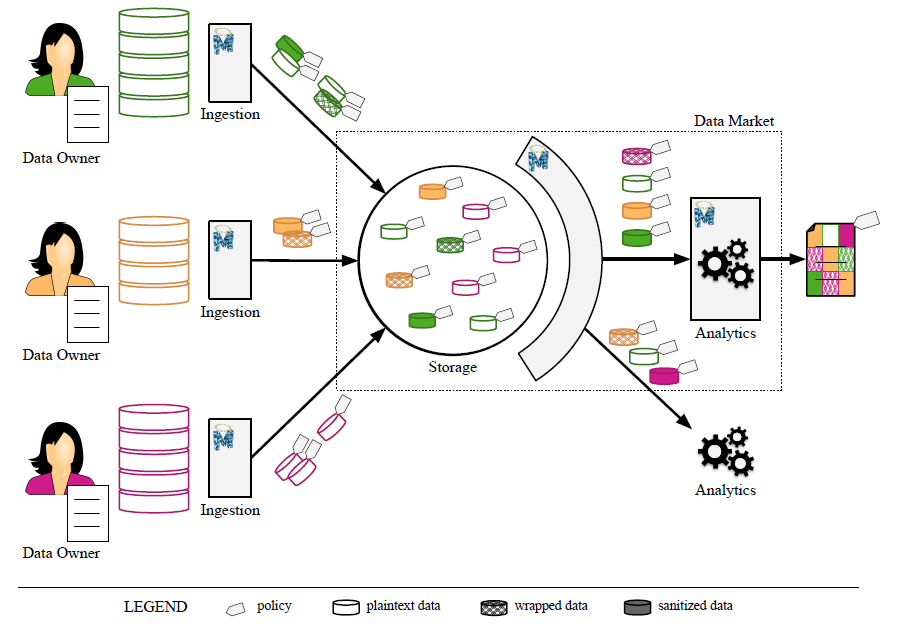
\includegraphics[width=1\linewidth]{images/i bellissimi dati.png}
\end{figure}
\begin{itemize}
    \item Nella fase di \textbf{ingestion} prendiamo i dati;
    \item in fase di \textbf{storage} li archiviamo con tutte le loro politiche, sanitizzati e/o wrappati
    \item e poi nell'ultima fase li \textbf{analizziamo} $ \rightarrow$ dovrebbero restare così come sono stati ceduti.
\end{itemize}
 

\end{document}